\section{Analiza pravilnosti}
\label{sec:analiza_pravilnosti}
V tem poglavju analiziramo pravilnost algoritma. Najprej predstavimo idejo testiranja, nato pa postopek ter rezultate. 

\subsection{Ideja testiranja}
Naj bo $\P$ množica nedominiranih točk, $\textbf{q}$ točka poizvedbe in $r$ z algoritmom izračunana razdalja $d(\textbf{q}, N(\P))$. Potem mora za vsak $\delta > 0$ veljati
\begin{align*}
    &S(\textbf{q}, r - \delta) \cap N(\P) = \varnothing, \\
    &S(\textbf{q}, r + \delta) \cap N(\P) \neq \varnothing,
\end{align*}
kjer je $S(\textbf{q}, r)$ sfera s središčem v $\textbf{q}$ in radijem $r$. 

Da lahko računamo presek sfere z $N(\P)$, sfero diskretiziramo. Diskretizacija sfere $S(\textbf{q}, r)$ je množica točk, označimo jo z $\Sigma(\textbf{q}, r, \varepsilon)$, ki ležijo na $S(\textbf{q}, r)$ in za katere velja
\[
\forall \textbf{x} \in S(\textbf{q}, r): \quad \min_{\textbf{s} \in \Sigma(\textbf{q}, r, \varepsilon)} ||\textbf{x} - \textbf{s}|| \leq \varepsilon.
\]
Presek med diskretno sfero $\Sigma(\textbf{q}, r)$ in $N(\P)$ izračunamo enostavno
\[
\Sigma(\textbf{q}, r, \varepsilon) \cap N(\P) = \{ \textbf{s} \in \Sigma(\textbf{q}, r, \varepsilon) \mid \textbf{s} \succeq 0 \land \neg  (\P \ggcurly \textbf{s}) \}.
\]
Opazimo tudi, da so vse komponente vektorja med poljubno točko $\textbf{q} \notin N(\P)$ in njej najbližjo točko $\textbf{z} \in N(\P)$ vedno nenegativne. Torej zadošča da preverimo le del sfere $\Sigma(\textbf{q}, r, \varepsilon)$, kjer so vsi elementi nenegativni, kar označimo s $\Sigma^+(\textbf{q}, r, \varepsilon)$.
Primer treh točk poizvedbe in ustrezajočih pozitivnih delov sfer vidimo na sliki~\ref{fig:test_example}.
\begin{figure}[ht]
  \centering
  \begin{tikzpicture}
    
    % Shade the non-dominated area (above and right)
    \fill[fillcol] 
        (0,5) -- (0,4) -- (0.5,4) -- 
        (0.5,2.5) -- (1.5,2.5) -- 
        (1.5,2) -- (2,2) -- 
        (2,1.5) -- (3.5,1.5) -- 
        (3.5,0.5) -- (4,0.5) -- 
        (4,0) -- (5,0) -- (5,5) -- cycle;
    \node at (3.75,3.75) {\( N(\P) \)};


    % Draw lines from each point (downward and leftward)
    \draw (0.5,4) -- (0.5,2.5);  
    \draw (0.5,4) -- (0,4);      

    \draw (1.5,2.5) -- (1.5,2);  
    \draw (1.5,2.5) -- (0.5,2.5);

    \draw (2,2) -- (2,1.5);      
    \draw (2,2) -- (1.5,2);      

    \draw (3.5,1.5) -- (3.5,0.5);
    \draw (3.5,1.5) -- (2,1.5);  

    \draw (4,0.5) -- (4,0);      
    \draw (4,0.5) -- (3.5,0.5);  

    % Nondominated points
    \fill (0.5,4) circle (2pt) node[above right] {\( \textbf{p}^1 \)};
    \fill (1.5,2.5) circle (2pt) node[above right] {\( \textbf{p}^2 \)};
    \fill (2,2) circle (2pt) node[above right] {\( \textbf{p}^3 \)};
    \fill (3.5,1.5) circle (2pt) node[above right] {\( \textbf{p}^4 \)};
    \fill (4,0.5) circle (2pt) node[above right] {\( \textbf{p}^5 \)};

    % Additional points q1, q2, q3
    \fill[nodecol2] (-0.4,4.2) circle (2pt) node[below left] {\( \textbf{q}^1 \)};
    \draw[nodecol, dashed] (-0.4,4.2) ++(0:0.45) arc[start angle=0, end angle=360, radius=0.45];    
    \draw[nodecol, dotted] (-0.4,4.2) ++(0:0.35) arc[start angle=0, end angle=360, radius=0.35];    


    
    \fill[nodecol2] (0.6,1) circle (2pt) node[below left] {\( \textbf{q}^2 \)};
    \draw[nodecol, dashed] (0.6,1) ++(0:1.3453624 + 0.05) arc[start angle=0, end angle=360, radius=1.3453624 + 0.05];    
    \draw[nodecol, dotted] (0.6,1) ++(0:1.3453624 - 0.05) arc[start angle=0, end angle=360, radius=1.3453624 - 0.05];    

    
    \fill[nodecol2] (2.5,1) circle (2pt) node[below left] {\( \textbf{q}^3 \)};
    \draw[nodecol, dashed] (2.5,1) ++(0:0.55) arc[start angle=0, end angle=360, radius=0.55];    
    \draw[nodecol, dotted] (2.5,1) ++(0:0.45) arc[start angle=0, end angle=360, radius=0.45];    
    
    % Draw lines to the nearest boundary of the non-dominated region
    \draw[nodecol2] (-0.4,4.2) -- (0,4.2);  % q1 to shaded region (horizontally right)
    \draw[nodecol2] (0.6, 1) -- (1.5,2);  % q2 to v (diagonal)
    \draw[nodecol2] (2.5,1) -- (2.5,1.5);  % q3 to shaded region (vertically up)

    % Draw axes
    \draw[->] (0,0) -- (5,0) node[midway, below] {\( f_1 \)};
    \draw[->] (0,0) -- (0,5) node[midway, left] {\( f_2 \)};
    
    % Draw a small dot at the origin
    \fill (0,0) circle (2pt);

\end{tikzpicture}

  \caption{Tri točke poizvedbe $\textbf{q}^1$, $\textbf{q}^2$, $\textbf{q}^3$ skupaj z njihovimi razdaljami do nedominiranega območja ter ustrezajočimi sferami $\Sigma^+(\textbf{q}, r + \delta, \varepsilon)$ s polno črto in $\Sigma^+(\textbf{q}, r - \delta, \varepsilon)$ s črtkano črto.}
  \label{fig:test_example}
\end{figure}

\subsection{Diskretizacija sfere}

%\nace{Nisem našel članka, ki bi razložil metodo s kocko, kot sva govorila v petek, da bi lahko samo enostavno citiral (morda ne iščem pravih ključnih besed). Prav trivialno se mi pa tudi ne zdi, tako da sem potem raje poskusil formalizirati algoritem, ki sem ga do zdaj uporabljal. Napisano (še) ni najbolje, ampak iz slik boste verjetno razumeli kaj je ideja. Povejte če se vam zdi ali je to v redu pristop, ker pri višjih dimenzijah težko argumentiram, da je to gotovo $\varepsilon$-net (kar sem uspel testirati zgleda sicer ok).}

%V tem razdelku predstavimo algoritem za diskretizacijo pozitivnega dela sfere. Brez škode za splošnost predpostavimo, da je središče sfere v $\textbf{0}$ in radij enak $1$, torej iščemo množico točk $\Sigma^+(\textbf{0}, 1)$, ki jo bomo v tem razdelku krajše imenovali $S^D$, kjer $D$ označuje dimenzijo sfere\footnote{Kot je običajno, bomo s $S^D$ mislili množico točk v $(D+1)$-dimenzionalnem prostoru}. Prav tako bomo tekom razdelka namesto `pozitivni del sfere' pisali le `sfera'.

%Algoritem rekurzivno deli sfero $S^D$ na več sfer manjše dimenzije $S^{d-1}$, dokler ne pride do $S^1$, kjer sfero razdeli na množico točk. Primer delitve sfere v $S^2$ na sfere $S^1$ je viden na sliki~\ref{fig:constructing_sphere_1}, primer delitev dveh sfer $S^1$ na točke pa je prikazan na sliki~\ref{fig:constructing_sphere_2}. Vidimo, da sfer ne razdelimo na enako število točk (oziroma sfer nižje dimenzije), temveč jih razdelimo tako, da so točke (oziroma sfere) čim bolj enakomerno razporejene. Tako poskrbimo, da je gostota točk po vsej sferi čim bolj enakomerna. 

\begin{figure}[ht]
    \begin{subfigure}{0.49\textwidth}
        \centering
        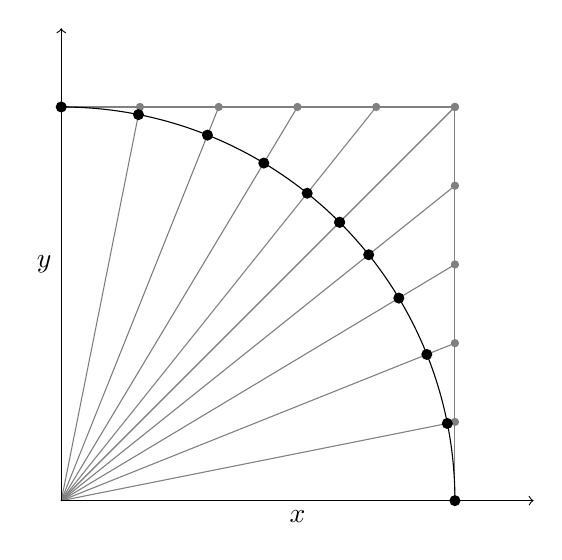
\begin{tikzpicture}

    \draw[gray] (5,0) -- (5,5);
    \draw[gray] (0,5) -- (5,5);

    \foreach \x in {0,1,2,3,4,5} {
        \draw[gray] (\x,5) -- (0,0);    
        \draw[gray] (5,\x) -- (0,0);    
        \fill[gray] (\x,5) circle (1.5pt);
        \fill[gray] (5,\x) circle (1.5pt);

        \pgfmathsetmacro{\r}{sqrt(\x*\x + 25)}
        \pgfmathsetmacro{\projx}{\x / \r * 5}
        \pgfmathsetmacro{\projy}{5 / \r * 5}

        \fill (\projx,\projy) circle (2pt);
        \fill (\projy,\projx) circle (2pt); 
    }

    \draw (5,0) arc[start angle=0, end angle=90, radius=5];    

    % Draw axes
    \draw[->] (0,0) -- (6,0) node[midway, below] {\( x \)};
    \draw[->] (0,0) -- (0,6) node[midway, left] {\( y \)};
\end{tikzpicture}

        \caption{Delitev sfere $S^2$ na 10 sfer $S^1$ označenih z debelejšo črto.}
        \label{fig:constructing_sphere_1}
    \end{subfigure}
    \hfill
    \begin{subfigure}{0.49\textwidth}
        \centering
        \tdplotsetmaincoords{70}{110}

\begin{tikzpicture}[scale=4,tdplot_main_coords]
\coordinate (O) at (0,0,0);
\draw[-stealth] (0,0,0) -- (1.2,0,0) node[anchor=north east]{$x$};
\draw[-stealth](0,0,0) -- (0,1.2,0) node[anchor=north west]{$y$};
\draw[-stealth] (0,0,0) -- (0,0,1.2) node[anchor=south]{$z$};

\draw[gray] (1,0,0) -- (1,1,0);
\draw[gray] (1,0,0) -- (1,0,1);
\draw[gray] (0,1,0) -- (1,1,0);
\draw[gray] (0,1,0) -- (0,1,1);
\draw[gray] (0,0,1) -- (1,0,1);
\draw[gray] (0,0,1) -- (0,1,1);
\draw[gray] (1,1,1) -- (0,1,1);
\draw[gray] (1,1,1) -- (1,0,1);
\draw[gray] (1,1,1) -- (1,1,0);

\foreach \x in {0,0.2,0.4,0.6,0.8,1} {
    \foreach \y in {0,0.2,0.4,0.6,0.8,1} {
        %\fill[gray] (\x,\y,1) circle (0.4pt);
        %\fill[gray] (\x,1,\y) circle (0.4pt);
        %\fill[gray] (1,\x,\y) circle (0.4pt);
        
        \pgfmathsetmacro{\r}{sqrt(\x*\x + \y*\y + 1)}
        \pgfmathsetmacro{\projx}{\x / \r}
        \pgfmathsetmacro{\projy}{\y / \r}
        \pgfmathsetmacro{\projz}{1 / \r}

        \draw[gray] (\projx,\projy,\projz) -- (\x,\y,1);
        \draw[gray] (\projx,\projz,\projy) -- (\x,1,\y);
        \draw[gray] (\projz,\projx,\projy) -- (1,\x,\y);

        \fill (\projx,\projy,\projz) circle (0.4pt);
        \fill (\projx,\projz,\projy) circle (0.4pt);
        \fill (\projz,\projx,\projy) circle (0.4pt);

        
    }
}






\tdplotsetthetaplanecoords{90}
% \tdplotdrawarc[tdplot_rotated_coords]{(0,0,0)}{0.5}{80}%
% {90}{anchor=west}{$d\phi_1$}
\draw[gray, dashed,tdplot_rotated_coords] (1,0,0) arc (0:90:1);

\draw[gray, dashed] (1,0,0) arc (0:90:1);

\tdplotsetthetaplanecoords{0}
\draw[gray, dashed,tdplot_rotated_coords] (1,0,0) arc (0:90:1);


\end{tikzpicture}
        \caption{Delitev dveh sfer $S^1$. Zgornjo razdelimo na 6 točk, spodnjo pa na 10 točk.}
        \label{fig:constructing_sphere_2}
    \end{subfigure}
    \caption{Prikaz delitve sfere $S^2$ na levi in sfere $S^1$ na desni.}
    \label{fig:constructing_sphere}
\end{figure}

Bolj formalno za sfero $S^D$ definiramo množico kotov $\{\phi^D_i\}_{i=0}^k$ kjer je $\phi_i = \frac{i}{k}\frac{\pi}{2}$ in je $k = \left\lceil \frac{\pi}{2 (\eta+1)} \right\rceil$. Spremenljivka $\eta$ predstavlja želeni razmik med točkami na sferi in je odvisna od izbire $\varepsilon$ ter dimenzije $D$. Primer za sfero $S^2$ je prikazan na sliki~\ref{fig:proof_h}, za splošen $D$, pa se izračuna kot:
\[
\eta = \frac{2 \varepsilon}{\sqrt{D}}.
\]
\begin{figure}[ht]
  \centering
  \input{tikz_images/proof_h}
  \caption{Skica prikazuje odvisnost $\eta$ od $\varepsilon$ v primeru sfere $S^2$. S črtkano črto sta predstavljeni dve sferi $S^1$, s črnimi pikami pa točke diskretizacije. Točka $\textbf{x}$ predstavlja točko, ki je od diskretizacije čim bolj oddaljena. \nace{tu zdaj predpostavljamo, da je sfera `lokalno ravna', kar nisem prepričan če je čisto v redu.}}
  \label{fig:proof_h}
\end{figure}

Za vsak kot $\phi_i$, definiramo sfero $S^{D-1}_i$, dimenzije $D-1$. Vsem točkam na sferi $S^{D-1}_i$ določimo zadnjo koordinato kot $\sin(\phi^D_i)$, vse ostale koordinate pa pomnožimo s $\cos(\phi^D_i)$. Ker so nove sfere $S^{D-1}_i$ različnih velikosti, moramo za vsako izmed njih ustrezno zmanjšati $k$, ki se na naslednjem koraku izračuna kot $k_i = \left\lceil \cos(\phi^{D}_i) \frac{\pi}{2 (\eta+1)} \right\rceil$.

Primer diskretizacije sfer $S^1$ in $S^2$, dobljenih z opisanim algoritmom, vidimo na sliki~\ref{fig:epsilon_net}.

\begin{figure}[ht]
    \begin{subfigure}{0.45\textwidth}
        \centering
        \begin{tikzpicture}
  \begin{axis}[
    xlabel={$f_1$},
    ylabel={$f_2$},
    xmin=0, xmax=3.5,
    ymin=0, ymax=3.5,
    width=6cm,
    height=6cm,
    enlargelimits=true,
    axis lines=middle,
    ticks=none
  ]
    \addplot[
      only marks,
      mark=*,
      black
    ] table [x=x, y=y, col sep=comma] {csv/epsilon_net_2D.csv};
  \end{axis}
\end{tikzpicture}

        \caption{Diskretna predstavitev $S^+_{0.2}(\textbf{0}, 3)$ v dveh dimenzijah vsebuje 14 točk.}
        \label{fig:epsilon_net_2d}
    \end{subfigure}
    \hfill
    \begin{subfigure}{0.45\textwidth}
        \centering
        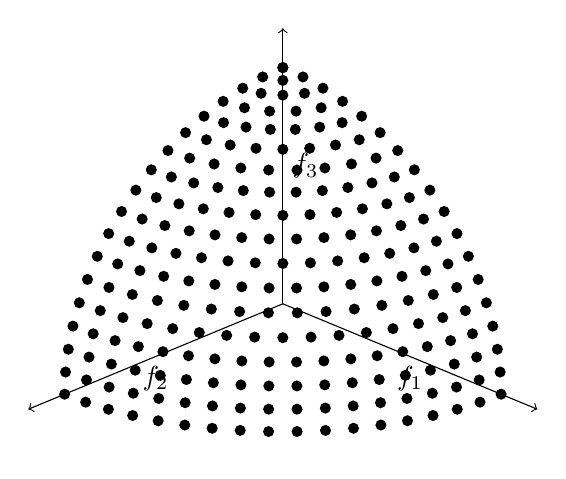
\begin{tikzpicture}
    % lines:
    % points:
    \fill[black] (2.77163859753386,-1.1480502970952693) circle (2pt) node[below left] {\(  \)};
    \fill[black] (2.5040807294832863,-1.2490816344177649) circle (2pt) node[below left] {\(  \)};
    \fill[black] (2.215158927562759,-1.3394562476491871) circle (2pt) node[below left] {\(  \)};
    \fill[black] (1.907338170715305,-1.4184030924546378) circle (2pt) node[below left] {\(  \)};
    \fill[black] (1.5832446771038056,-1.4852486221901098) circle (2pt) node[below left] {\(  \)};
    \fill[black] (1.245643498143606,-1.5394225343649701) circle (2pt) node[below left] {\(  \)};
    \fill[black] (0.8974149280587729,-1.5804626362617262) circle (2pt) node[below left] {\(  \)};
    \fill[black] (0.5415299302273326,-1.6080187882013268) circle (2pt) node[below left] {\(  \)};
    \fill[black] (0.1810247899692694,-1.6218558908114495) circle (2pt) node[below left] {\(  \)};
    \fill[black] (-0.1810247899692694,-1.6218558908114495) circle (2pt) node[below left] {\(  \)};
    \fill[black] (-0.5415299302273326,-1.6080187882013268) circle (2pt) node[below left] {\(  \)};
    \fill[black] (-0.897414928058772,-1.580462636261726) circle (2pt) node[below left] {\(  \)};
    \fill[black] (-1.245643498143606,-1.5394225343649701) circle (2pt) node[below left] {\(  \)};
    \fill[black] (-1.5832446771038053,-1.48524862219011) circle (2pt) node[below left] {\(  \)};
    \fill[black] (-1.9073381707153052,-1.4184030924546378) circle (2pt) node[below left] {\(  \)};
    \fill[black] (-2.215158927562759,-1.3394562476491871) circle (2pt) node[below left] {\(  \)};
    \fill[black] (-2.5040807294832863,-1.2490816344177649) circle (2pt) node[below left] {\(  \)};
    \fill[black] (-2.77163859753386,-1.1480502970952693) circle (2pt) node[below left] {\(  \)};
    \fill[black] (2.759815275902903,-0.8663478385335218) circle (2pt) node[below left] {\(  \)};
    \fill[black] (2.493398762548309,-0.966948193982322) circle (2pt) node[below left] {\(  \)};
    \fill[black] (2.2057094500992958,-1.056937285046295) circle (2pt) node[below left] {\(  \)};
    \fill[black] (1.8992018023332822,-1.1355473565297425) circle (2pt) node[below left] {\(  \)};
    \fill[black] (1.576490834429456,-1.202107735019898) circle (2pt) node[below left] {\(  \)};
    \fill[black] (1.2403298025812892,-1.256050550836012) circle (2pt) node[below left] {\(  \)};
    \fill[black] (0.8935867141854699,-1.2969155828932424) circle (2pt) node[below left] {\(  \)};
    \fill[black] (0.5392198590140203,-1.3243541851466816) circle (2pt) node[below left] {\(  \)};
    \fill[black] (0.18025257012903206,-1.338132261116482) circle (2pt) node[below left] {\(  \)};
    \fill[black] (-0.18025257012903206,-1.338132261116482) circle (2pt) node[below left] {\(  \)};
    \fill[black] (-0.5392198590140203,-1.3243541851466816) circle (2pt) node[below left] {\(  \)};
    \fill[black] (-0.893586714185469,-1.2969155828932424) circle (2pt) node[below left] {\(  \)};
    \fill[black] (-1.2403298025812892,-1.256050550836012) circle (2pt) node[below left] {\(  \)};
    \fill[black] (-1.5764908344294555,-1.202107735019898) circle (2pt) node[below left] {\(  \)};
    \fill[black] (-1.8992018023332822,-1.1355473565297425) circle (2pt) node[below left] {\(  \)};
    \fill[black] (-2.2057094500992958,-1.056937285046295) circle (2pt) node[below left] {\(  \)};
    \fill[black] (-2.493398762548309,-0.966948193982322) circle (2pt) node[below left] {\(  \)};
    \fill[black] (-2.759815275902903,-0.8663478385335218) circle (2pt) node[below left] {\(  \)};
    \fill[black] (2.7244461834214007,-0.5772540056790502) circle (2pt) node[below left] {\(  \)};
    \fill[black] (2.461443996518912,-0.6765650924921532) circle (2pt) node[below left] {\(  \)};
    \fill[black] (2.177441637318833,-0.7654009061929788) circle (2pt) node[below left] {\(  \)};
    \fill[black] (1.874862113813446,-0.843003530941656) circle (2pt) node[below left] {\(  \)};
    \fill[black] (1.5562869278107652,-0.9087108885057454) circle (2pt) node[below left] {\(  \)};
    \fill[black] (1.224434050471319,-0.9619623868782713) circle (2pt) node[below left] {\(  \)};
    \fill[black] (0.8821347335365373,-1.0023037030510689) circle (2pt) node[below left] {\(  \)};
    \fill[black] (0.5323093540871684,-1.0293906591384987) circle (2pt) node[below left] {\(  \)};
    \fill[black] (0.17794249891572012,-1.0429921587818156) circle (2pt) node[below left] {\(  \)};
    \fill[black] (-0.17794249891572012,-1.0429921587818156) circle (2pt) node[below left] {\(  \)};
    \fill[black] (-0.5323093540871684,-1.0293906591384987) circle (2pt) node[below left] {\(  \)};
    \fill[black] (-0.8821347335365368,-1.0023037030510689) circle (2pt) node[below left] {\(  \)};
    \fill[black] (-1.2244340504713187,-0.9619623868782715) circle (2pt) node[below left] {\(  \)};
    \fill[black] (-1.5562869278107652,-0.9087108885057457) circle (2pt) node[below left] {\(  \)};
    \fill[black] (-1.874862113813446,-0.843003530941656) circle (2pt) node[below left] {\(  \)};
    \fill[black] (-2.1774416373188332,-0.7654009061929786) circle (2pt) node[below left] {\(  \)};
    \fill[black] (-2.461443996518912,-0.6765650924921532) circle (2pt) node[below left] {\(  \)};
    \fill[black] (-2.7244461834214007,-0.5772540056790502) circle (2pt) node[below left] {\(  \)};
    \fill[black] (2.6658330767156153,-0.2832352451821549) circle (2pt) node[below left] {\(  \)};
    \fill[black] (2.408489058191924,-0.3804097761829739) circle (2pt) node[below left] {\(  \)};
    \fill[black] (2.1305966602330626,-0.4673343966807817) circle (2pt) node[below left] {\(  \)};
    \fill[black] (1.8345267627963162,-0.543267496462249) circle (2pt) node[below left] {\(  \)};
    \fill[black] (1.52280532985531,-0.6075612410932971) circle (2pt) node[below left] {\(  \)};
    \fill[black] (1.198091858766014,-0.6596670990140701) circle (2pt) node[below left] {\(  \)};
    \fill[black] (0.8631566903730181,-0.6991405214167954) circle (2pt) node[below left] {\(  \)};
    \fill[black] (0.520857373438236,-0.7256447349794697) circle (2pt) node[below left] {\(  \)};
    \fill[black] (0.17411428504241688,-0.7389536150970994) circle (2pt) node[below left] {\(  \)};
    \fill[black] (-0.17411428504241688,-0.7389536150970994) circle (2pt) node[below left] {\(  \)};
    \fill[black] (-0.520857373438236,-0.7256447349794697) circle (2pt) node[below left] {\(  \)};
    \fill[black] (-0.8631566903730179,-0.6991405214167954) circle (2pt) node[below left] {\(  \)};
    \fill[black] (-1.198091858766014,-0.6596670990140701) circle (2pt) node[below left] {\(  \)};
    \fill[black] (-1.5228053298553095,-0.6075612410932973) circle (2pt) node[below left] {\(  \)};
    \fill[black] (-1.8345267627963162,-0.543267496462249) circle (2pt) node[below left] {\(  \)};
    \fill[black] (-2.1305966602330626,-0.4673343966807817) circle (2pt) node[below left] {\(  \)};
    \fill[black] (-2.408489058191924,-0.3804097761829741) circle (2pt) node[below left] {\(  \)};
    \fill[black] (-2.6658330767156153,-0.2832352451821549) circle (2pt) node[below left] {\(  \)};
    \fill[black] (2.584476022145561,0.013199978560699988) circle (2pt) node[below left] {\(  \)};
    \fill[black] (2.3187081147487505,-0.08657495197546461) circle (2pt) node[below left] {\(  \)};
    \fill[black] (2.03060978067212,-0.17507925423692972) circle (2pt) node[below left] {\(  \)};
    \fill[black] (1.7229555643633956,-0.251460583411544) circle (2pt) node[below left] {\(  \)};
    \fill[black] (1.398708344106534,-0.314983345545075) circle (2pt) node[below left] {\(  \)};
    \fill[black] (1.060990797884168,-0.36503578171310225) circle (2pt) node[below left] {\(  \)};
    \fill[black] (0.7130553302816098,-0.40113585959388254) circle (2pt) node[below left] {\(  \)};
    \fill[black] (0.35825275005274615,-0.42293591570311473) circle (2pt) node[below left] {\(  \)};
    \fill[black] (0.0,-0.4302260035833434) circle (2pt) node[below left] {\(  \)};
    \fill[black] (-0.3582527500527457,-0.4229359157031143) circle (2pt) node[below left] {\(  \)};
    \fill[black] (-0.7130553302816098,-0.40113585959388254) circle (2pt) node[below left] {\(  \)};
    \fill[black] (-1.060990797884167,-0.36503578171310225) circle (2pt) node[below left] {\(  \)};
    \fill[black] (-1.3987083441065338,-0.31498334554507523) circle (2pt) node[below left] {\(  \)};
    \fill[black] (-1.722955564363396,-0.2514605834115442) circle (2pt) node[below left] {\(  \)};
    \fill[black] (-2.03060978067212,-0.17507925423692972) circle (2pt) node[below left] {\(  \)};
    \fill[black] (-2.31870811474875,-0.08657495197546461) circle (2pt) node[below left] {\(  \)};
    \fill[black] (-2.584476022145561,0.013199978560699988) circle (2pt) node[below left] {\(  \)};
    \fill[black] (2.4810691294151392,0.3095225847406564) circle (2pt) node[below left] {\(  \)};
    \fill[black] (2.208135229767077,0.207729275772774) circle (2pt) node[below left] {\(  \)};
    \fill[black] (1.911008538459683,0.11831084949728554) circle (2pt) node[below left] {\(  \)};
    \fill[black] (1.592944437700678,0.04224699290447442) circle (2pt) node[below left] {\(  \)};
    \fill[black] (1.257427704337171,-0.019628922475444233) circle (2pt) node[below left] {\(  \)};
    \fill[black] (0.9081343299112821,-0.06663897116519935) circle (2pt) node[below left] {\(  \)};
    \fill[black] (0.5488912457275592,-0.09826810123386132) circle (2pt) node[below left] {\(  \)};
    \fill[black] (0.18363439419276828,-0.11416977731357658) circle (2pt) node[below left] {\(  \)};
    \fill[black] (-0.18363439419276717,-0.11416977731357658) circle (2pt) node[below left] {\(  \)};
    \fill[black] (-0.5488912457275592,-0.09826810123386132) circle (2pt) node[below left] {\(  \)};
    \fill[black] (-0.9081343299112812,-0.06663897116519957) circle (2pt) node[below left] {\(  \)};
    \fill[black] (-1.2574277043371709,-0.019628922475444455) circle (2pt) node[below left] {\(  \)};
    \fill[black] (-1.5929444377006778,0.0422469929044742) circle (2pt) node[below left] {\(  \)};
    \fill[black] (-1.9110085384596824,0.11831084949728554) circle (2pt) node[below left] {\(  \)};
    \fill[black] (-2.208135229767076,0.20772927577277378) circle (2pt) node[below left] {\(  \)};
    \fill[black] (-2.4810691294151392,0.3095225847406564) circle (2pt) node[below left] {\(  \)};
    \fill[black] (2.3564946296728837,0.6032044533621944) circle (2pt) node[below left] {\(  \)};
    \fill[black] (2.0972647431892493,0.5065221872070418) circle (2pt) node[below left] {\(  \)};
    \fill[black] (1.8150567852983701,0.42159346079075677) circle (2pt) node[below left] {\(  \)};
    \fill[black] (1.5129626854427112,0.3493487710124348) circle (2pt) node[below left] {\(  \)};
    \fill[black] (1.1942922497975463,0.29057964581146) circle (2pt) node[below left] {\(  \)};
    \fill[black] (0.8625368983418786,0.24592997202176492) circle (2pt) node[below left] {\(  \)};
    \fill[black] (0.5213314121305272,0.21588894081293386) circle (2pt) node[below left] {\(  \)};
    \fill[black] (0.1744141098722627,0.20078568800938124) circle (2pt) node[below left] {\(  \)};
    \fill[black] (-0.17441410987226225,0.20078568800938124) circle (2pt) node[below left] {\(  \)};
    \fill[black] (-0.5213314121305272,0.21588894081293386) circle (2pt) node[below left] {\(  \)};
    \fill[black] (-0.8625368983418777,0.24592997202176492) circle (2pt) node[below left] {\(  \)};
    \fill[black] (-1.1942922497975457,0.2905796458114598) circle (2pt) node[below left] {\(  \)};
    \fill[black] (-1.512962685442711,0.3493487710124348) circle (2pt) node[below left] {\(  \)};
    \fill[black] (-1.8150567852983692,0.421593460790757) circle (2pt) node[below left] {\(  \)};
    \fill[black] (-2.0972647431892484,0.5065221872070416) circle (2pt) node[below left] {\(  \)};
    \fill[black] (-2.3564946296728837,0.6032044533621943) circle (2pt) node[below left] {\(  \)};
    \fill[black] (2.2118153486268626,0.8917399942715472) circle (2pt) node[below left] {\(  \)};
    \fill[black] (1.9502631712135305,0.7949228279188589) circle (2pt) node[below left] {\(  \)};
    \fill[black] (1.664185302853139,0.7108444864078123) circle (2pt) node[below left] {\(  \)};
    \fill[black] (1.3571793387265654,0.6405623036662984) circle (2pt) node[below left] {\(  \)};
    \fill[black] (1.03310605696171,0.5849601189209643) circle (2pt) node[below left] {\(  \)};
    \fill[black] (0.6960408671084657,0.5447371619061212) circle (2pt) node[below left] {\(  \)};
    \fill[black] (0.3502225594990145,0.5203992596441345) circle (2pt) node[below left] {\(  \)};
    \fill[black] (0.0,0.5122524753771283) circle (2pt) node[below left] {\(  \)};
    \fill[black] (-0.35022255949901404,0.5203992596441345) circle (2pt) node[below left] {\(  \)};
    \fill[black] (-0.6960408671084655,0.5447371619061214) circle (2pt) node[below left] {\(  \)};
    \fill[black] (-1.03310605696171,0.5849601189209643) circle (2pt) node[below left] {\(  \)};
    \fill[black] (-1.3571793387265654,0.6405623036662984) circle (2pt) node[below left] {\(  \)};
    \fill[black] (-1.6641853028531388,0.7108444864078121) circle (2pt) node[below left] {\(  \)};
    \fill[black] (-1.9502631712135303,0.7949228279188589) circle (2pt) node[below left] {\(  \)};
    \fill[black] (-2.2118153486268626,0.891739994271547) circle (2pt) node[below left] {\(  \)};
    \fill[black] (2.0482656388904843,1.1726675239684405) circle (2pt) node[below left] {\(  \)};
    \fill[black] (1.7864403358437966,1.07658779790182) circle (2pt) node[below left] {\(  \)};
    \fill[black] (1.4985647099872053,0.9942809960217152) circle (2pt) node[below left] {\(  \)};
    \fill[black] (1.1888366361851541,0.9269473368383148) circle (2pt) node[below left] {\(  \)};
    \fill[black] (0.8617726472005588,0.8755686967247087) circle (2pt) node[below left] {\(  \)};
    \fill[black] (0.5221420724767789,0.8408942919483746) circle (2pt) node[below left] {\(  \)};
    \fill[black] (0.17489749057473647,0.8234297534109118) circle (2pt) node[below left] {\(  \)};
    \fill[black] (-0.1748974905747358,0.8234297534109114) circle (2pt) node[below left] {\(  \)};
    \fill[black] (-0.5221420724767785,0.8408942919483746) circle (2pt) node[below left] {\(  \)};
    \fill[black] (-0.8617726472005586,0.8755686967247085) circle (2pt) node[below left] {\(  \)};
    \fill[black] (-1.1888366361851532,0.9269473368383148) circle (2pt) node[below left] {\(  \)};
    \fill[black] (-1.498564709987205,0.9942809960217152) circle (2pt) node[below left] {\(  \)};
    \fill[black] (-1.7864403358437961,1.0765877979018197) circle (2pt) node[below left] {\(  \)};
    \fill[black] (-2.0482656388904843,1.1726675239684405) circle (2pt) node[below left] {\(  \)};
    \fill[black] (1.867240848921215,1.4435902678217585) circle (2pt) node[below left] {\(  \)};
    \fill[black] (1.6075425066427875,1.349253404999835) circle (2pt) node[below left] {\(  \)};
    \fill[black] (1.3203386663807173,1.2697643847315256) circle (2pt) node[below left] {\(  \)};
    \fill[black] (1.0105434654698358,1.2064832861921415) circle (2pt) node[below left] {\(  \)};
    \fill[black] (0.683457585689186,1.160492866522526) circle (2pt) node[below left] {\(  \)};
    \fill[black] (0.3446775571271523,1.13258003455418) circle (2pt) node[below left] {\(  \)};
    \fill[black] (0.0,1.1232223865809807) circle (2pt) node[below left] {\(  \)};
    \fill[black] (-0.34467755712715187,1.13258003455418) circle (2pt) node[below left] {\(  \)};
    \fill[black] (-0.6834575856891856,1.160492866522526) circle (2pt) node[below left] {\(  \)};
    \fill[black] (-1.0105434654698358,1.2064832861921415) circle (2pt) node[below left] {\(  \)};
    \fill[black] (-1.3203386663807164,1.2697643847315256) circle (2pt) node[below left] {\(  \)};
    \fill[black] (-1.6075425066427873,1.349253404999835) circle (2pt) node[below left] {\(  \)};
    \fill[black] (-1.8672408489212147,1.4435902678217585) circle (2pt) node[below left] {\(  \)};
    \fill[black] (1.67028541839953,1.7021968085056134) circle (2pt) node[below left] {\(  \)};
    \fill[black] (1.4155779220031643,1.610777679136545) circle (2pt) node[below left] {\(  \)};
    \fill[black] (1.1320533413044434,1.5353037496868345) circle (2pt) node[below left] {\(  \)};
    \fill[black] (0.8254834191490192,1.477311451711238) circle (2pt) node[below left] {\(  \)};
    \fill[black] (0.5021090350773254,1.4379813411605618) circle (2pt) node[below left] {\(  \)};
    \fill[black] (0.16851315901434538,1.4181140656669444) circle (2pt) node[below left] {\(  \)};
    \fill[black] (-0.16851315901434538,1.4181140656669444) circle (2pt) node[below left] {\(  \)};
    \fill[black] (-0.5021090350773251,1.437981341160562) circle (2pt) node[below left] {\(  \)};
    \fill[black] (-0.8254834191490188,1.477311451711238) circle (2pt) node[below left] {\(  \)};
    \fill[black] (-1.132053341304443,1.5353037496868343) circle (2pt) node[below left] {\(  \)};
    \fill[black] (-1.4155779220031643,1.610777679136545) circle (2pt) node[below left] {\(  \)};
    \fill[black] (-1.67028541839953,1.7021968085056134) circle (2pt) node[below left] {\(  \)};
    \fill[black] (1.4590797016141113,1.946280806196989) circle (2pt) node[below left] {\(  \)};
    \fill[black] (1.183546471156217,1.8505147001417144) circle (2pt) node[below left] {\(  \)};
    \fill[black] (0.8720517800756533,1.7760218936437986) circle (2pt) node[below left] {\(  \)};
    \fill[black] (0.5340602369369836,1.7250658129335017) circle (2pt) node[below left] {\(  \)};
    \fill[black] (0.17984154374650274,1.699194732738185) circle (2pt) node[below left] {\(  \)};
    \fill[black] (-0.17984154374650274,1.699194732738185) circle (2pt) node[below left] {\(  \)};
    \fill[black] (-0.5340602369369829,1.7250658129335017) circle (2pt) node[below left] {\(  \)};
    \fill[black] (-0.8720517800756529,1.7760218936437986) circle (2pt) node[below left] {\(  \)};
    \fill[black] (-1.183546471156217,1.8505147001417144) circle (2pt) node[below left] {\(  \)};
    \fill[black] (-1.4590797016141113,1.946280806196989) circle (2pt) node[below left] {\(  \)};
    \fill[black] (1.2354256312715333,2.1737598222891754) circle (2pt) node[below left] {\(  \)};
    \fill[black] (0.9706676899522468,2.0837589911569796) circle (2pt) node[below left] {\(  \)};
    \fill[black] (0.6686075336648074,2.0168823404003793) circle (2pt) node[below left] {\(  \)};
    \fill[black] (0.34085316481805417,1.9756999022030932) circle (2pt) node[below left] {\(  \)};
    \fill[black] (0.0,1.961794294569665) circle (2pt) node[below left] {\(  \)};
    \fill[black] (-0.34085316481805406,1.9756999022030932) circle (2pt) node[below left] {\(  \)};
    \fill[black] (-0.6686075336648074,2.0168823404003793) circle (2pt) node[below left] {\(  \)};
    \fill[black] (-0.9706676899522467,2.0837589911569796) circle (2pt) node[below left] {\(  \)};
    \fill[black] (-1.2354256312715333,2.1737598222891754) circle (2pt) node[below left] {\(  \)};
    \fill[black] (1.0012313450417556,2.3826930860237163) circle (2pt) node[below left] {\(  \)};
    \fill[black] (0.7533334508275297,2.3008063893051767) circle (2pt) node[below left] {\(  \)};
    \fill[black] (0.46766027174226815,2.243821806637896) circle (2pt) node[below left] {\(  \)};
    \fill[black] (0.15853665385261795,2.214596782943707) circle (2pt) node[below left] {\(  \)};
    \fill[black] (-0.15853665385261784,2.214596782943707) circle (2pt) node[below left] {\(  \)};
    \fill[black] (-0.4676602717422681,2.243821806637896) circle (2pt) node[below left] {\(  \)};
    \fill[black] (-0.7533334508275296,2.3008063893051767) circle (2pt) node[below left] {\(  \)};
    \fill[black] (-1.0012313450417556,2.3826930860237163) circle (2pt) node[below left] {\(  \)};
    \fill[black] (0.7584949060003102,2.5712980524622226) circle (2pt) node[below left] {\(  \)};
    \fill[black] (0.4869837068273508,2.489588448927818) circle (2pt) node[below left] {\(  \)};
    \fill[black] (0.1678031494151312,2.4466311681908617) circle (2pt) node[below left] {\(  \)};
    \fill[black] (-0.1678031494151312,2.4466311681908617) circle (2pt) node[below left] {\(  \)};
    \fill[black] (-0.4869837068273507,2.489588448927818) circle (2pt) node[below left] {\(  \)};
    \fill[black] (-0.7584949060003102,2.5712980524622226) circle (2pt) node[below left] {\(  \)};
    \fill[black] (0.509287255858642,2.7379656105312793) circle (2pt) node[below left] {\(  \)};
    \fill[black] (0.27562427672485545,2.6732950223268497) circle (2pt) node[below left] {\(  \)};
    \fill[black] (0.0,2.6505857317134893) circle (2pt) node[below left] {\(  \)};
    \fill[black] (-0.27562427672485545,2.6732950223268497) circle (2pt) node[below left] {\(  \)};
    \fill[black] (-0.509287255858642,2.7379656105312793) circle (2pt) node[below left] {\(  \)};
    \fill[black] (0.25573454641961646,2.8812738113907668) circle (2pt) node[below left] {\(  \)};
    \fill[black] (0.0,2.837396699959824) circle (2pt) node[below left] {\(  \)};
    \fill[black] (-0.25573454641961646,2.8812738113907668) circle (2pt) node[below left] {\(  \)};
    \fill[black] (1.6971391684315505e-16,3.0) circle (2pt) node[below left] {\(  \)};
    \fill[black] (-1.6971391684315505e-16,3.0) circle (2pt) node[below left] {\(  \)};
    % axes:
    \draw[->] (0.0,0.0) -- (3.2336,-1.3394) node[midway, below] {\( f_1 \)};
    \draw[->] (0.0,0.0) -- (-3.2336,-1.3394) node[midway, below] {\( f_2 \)};
    \draw[->] (0.0,0.0) -- (0.0,3.5) node[midway, right] {\( f_3 \)};
\end{tikzpicture}
        \caption{Diskretna predstavitev $S^+_{0.2}(\textbf{0}, 3)$ v treh dimenzijah vsebuje 218 točk.}
        \label{fig:epsilon_net_3d}
    \end{subfigure}
    \caption{Primera diskretizacij sfere $S^1$ v dvodimenzionalnem prostoru na levi in $S^2$ v tridimenzionalnem prostoru na desni. Pri obeh je $r=3$ ter $\varepsilon = 0.2$, vidimo pa, da je število točk precej večje pri $S^2$.}
    \label{fig:epsilon_net}
\end{figure}



\subsection{Testiranje}


\begin{figure}[ht]
    \begin{subfigure}{0.49\textwidth}
      \centering
      \begin{tikzpicture}
    
    % Shade the non-dominated area (above and right)
    \fill[fillcol] 
        (-2,4) -- (-2,3) -- (0,3) -- 
        (0, 0) -- (3,0) -- 
        (3, -1) -- (4,-1) -- (4,4) -- cycle;
    \node at (3,3) {\( N(\P) \)};


    % Draw lines from each point (downward and leftward)
    \draw (0,3) -- (-2,3);  
    \draw (0,3) -- (0,0);      

    \draw (3,0) -- (0,0);  
    \draw (3,0) -- (3, -1);  

    
    \fill (0,3) circle (2pt) node[above right] {\( \textbf{p}^i \)};
    \fill (3,0) circle (2pt) node[above right] {\( \textbf{p}^{i+1} \)};
    
     \fill (-2,-1) circle (2pt) node[above right] {\( \textbf{q} \)};
    \draw[nodecol, dashed] (-2,-1) -- (0.23606798,-1) node[midway, above] {$r$};  
    \draw[nodecol, dashed] (0.23606798,-1) -- (1.23606798,-1) node[midway, above] {$\delta$};
    \draw[nodecol] (1.23606798,-1) arc[start angle=0, end angle=90, radius=3.23606798];    
    \draw[nodecol, dashed] (0.23606798,-1) arc[start angle=0, end angle=90, radius=2.23606798];    
    \draw[blue, dashed] (-2,-1) -- (0,0);  
    \draw[blue] (0.8944272,0.4472136) -- (0,0) node[midway, right] {$\delta$};
    \draw[blue] (1, 0) arc[start angle=0, end angle=90, radius=1];    
    \fill[blue] (0.70710678,0.70710678) circle (1pt) node[left] {$\overline{\textbf{s}}$};
    
    
    \draw[gray, dashed] (1,1) -- (0,0);
    \fill[gray] (0.73295,0.73295) circle (1pt) node[right] {\( \textbf{s} \)};


    % % Additional points q1, q2, q3
    % \fill[nodecol2] (-0.4,4.2) circle (2pt) node[below left] {\( \textbf{q}^1 \)};
    % \draw[nodecol] (-0.4,4.2) ++(0:0.45) arc[start angle=0, end angle=90, radius=0.45];    
    % \draw[nodecol, dashed] (-0.4,4.2) ++(0:0.35) arc[start angle=0, end angle=90, radius=0.35];    


    
    % \fill[nodecol2] (0.5,1) circle (2pt) node[below left] {\( \textbf{q}^2 \)};
    % \draw[nodecol] (0.5,1) ++(0:1.414 + 0.05) arc[start angle=0, end angle=90, radius=1.414 + 0.05];    
    % \draw[nodecol, dashed] (0.5,1) ++(0:1.414 - 0.05) arc[start angle=0, end angle=90, radius=1.414 - 0.05];    

    
    % \fill[nodecol2] (2.5,1) circle (2pt) node[below left] {\( \textbf{q}^3 \)};
    % \draw[nodecol, dashed] (2.5,1) ++(0:0.45) arc[start angle=0, end angle=90, radius=0.45];    
    
    % % Draw lines to the nearest boundary of the non-dominated region
    % \draw[nodecol2] (-0.4,4.2) -- (0,4.2);  % q1 to shaded region (horizontally right)
    % \draw[nodecol2] (0.5, 1) -- (1.5,2);  % q2 to v (diagonal)
    % \draw[nodecol2] (2.5,1) -- (2.5,1.5);  % q3 to shaded region (vertically up)

    % % Draw axes
    % \draw[->] (0,0) -- (5,0) node[midway, below] {\( f_1 \)};
    % \draw[->] (0,0) -- (0,5) node[midway, left] {\( f_2 \)};
    
    % % Draw a small dot at the origin
    % \fill (0,0) circle (2pt);

\end{tikzpicture}

      \caption{Slika prikazuje ilustracijo testne sfere z izhodiščem v $q$ in radijem $r+\delta$ s polno oranžno črto, ki vsebuje modro sfero z izhodiščem v vpeti točki. Za izbiro $\varepsilon = \frac{\delta}{2} (?)$ tako velja, da bo vsaj ena točka diskretizacije testne sfere znotraj $N(\P)$.}
      \label{fig:determining-epsilon1}
    \end{subfigure}
    \hfill
    \begin{subfigure}{0.49\textwidth}
      \centering
      \begin{tikzpicture}
    
    % Shade the non-dominated area (above and right)
    \fill[fillcol] 
        (-2,4) -- (-2,3) -- (0.1,3) -- 
        (0.1, 0) -- (3,0) -- 
        (3, -1) -- (4,-1) -- (4,4) -- cycle;
    \node at (3,3) {\( N(\P) \)};


    % Draw lines from each point (downward and leftward)
    \draw (0.1,3) -- (-2,3);  
    \draw (0.1,3) -- (0.1,0);      

    \draw (3,0) -- (0.1,0);  
    \draw (3,0) -- (3, -1);  

    
    \fill (0.1,3) circle (2pt) node[above right] {\( \textbf{p}^i \)};
    \fill (3,0) circle (2pt) node[above right] {\( \textbf{p}^{i+1} \)};
    
     \fill (-2,-1) circle (2pt) node[above right] {\( \textbf{q} \)};
    \draw[nodecol, dashed] (-2,-1) -- (0.5,-1) node[midway, above] {$r$};  
    \draw[nodecol, dashed] (-2,-1) -- (-2,1.5);  
    \draw[nodecol] (0.5,-1) arc[start angle=0, end angle=90, radius=2.5];

    \foreach \x in {0, 18, 36, 54, 72, 90} {
        \fill[nodecol] ({-2 + 2.5* cos(\x)}, {-1 + 2.5* sin(\x)}) circle (2pt);
    }

    


\end{tikzpicture}

      \caption{Slika prikazuje diskretizacijo testne sfere z izhodiščem v $q$ in radijem $r-\delta'$, kjer je $r$ napačno izračunana razdalja algoritma. Želimo si, da bi bila diskretizacija testne sfere dovolj gosta, da bi se vsaj ena izmed točk nahajala v $N(\P)$, za vsak $r > \delta + d(\textbf{q}, N(\P))$}
      \label{fig:determining-epsilon3}
    \end{subfigure}
    \caption{Sliki prikazujeta kako določimo epsilon kadar želimo pokazati, da je $d(\textbf{q}, N(\P)) < r + \delta$ (na sliki a) in $r - \delta < d(\textbf{q}, N(\P))$ (na sliki b).}
    \label{fig:determining-epsilon}
\end{figure}




